\documentclass[11pt]{article}
\usepackage[utf8]{inputenc}
\usepackage[english]{babel}
\usepackage{amsfonts}
\usepackage{amssymb}
\usepackage{amsmath}
\usepackage{graphicx}
\usepackage{array}
\usepackage{float}
\usepackage{lipsum}
\usepackage{tikz}
\begin{document}
\title{PS239T Final Project Report: \\Discussion on Constitution Issues \\ in the Hong Kong LegCo}
\author{Chuyue Frances Huang}
\date{December 12, 2016}
\maketitle
\section*{Background}
As Hong Kong is about to host its election for chief executive in March 2017, the tension within the Hong Kong Legislative Council (abbreviated as “LegCo”) is growing. Recently, two legislators-elect from the Youngspiration party have been disqualified for supporting Hong Kong independence under oath. This recent development makes LeCo a key place for debate on consitutional issues. \par
The relationship between Hong Kong and China is governed by the "Basic Law," which is equivalenet to the constitution of Hong Kong. Yet it does not specify whether or not Hong Kong can hold free and fair elections, and specific provision are subject to Beijing's interpretation. Therefore, the key here is to see if how the discussion on these key constitutional matters have progressed in the past 19 years. 

\section*{Research Questions}
By completing this project, I want to answer these following questions. First, how has the effectiveness of governance changein Hong Kong since 1997? Is Hong Kong getting closing to becoming a democracy? Second, how has the discussion on key constitutional and electoral matters change in the past 19 years? If so, who are the most active legislators behind the discussions? Are these members from the pan-democracy alliance really behind the discussions? 

\section*{Data and Skills}
To answer the first question, I collected the data from the World Bank, which includes a list of indicators for governance effectiveness. I then obtained a table with countries and their regions. \par
To answer the second question, I used the HK Legco open database for a list of council events on the six issues that fall under the catergory of "Constitutional Affairs." In particular, the more relevant sub-issues are press freedom, electoral matters and consitutional development. Using regex and extractMatches(), I extracted the names of the names of the members and the names of the motions from the summary variable. \par 
To get the names of the members, their parties and the affiliation of the parties (Pro-Beijing or Pan-democracy), I used XML to scrape the table from Wikipedia. Then I merged the table with the party information to the one with the council events. Lastly, I used wordcloud and ggplot to visualize the number of actions on the key policy issues and the key terms in the motions. 
\section*{Result}
\begin{figure}[H]
	\centering
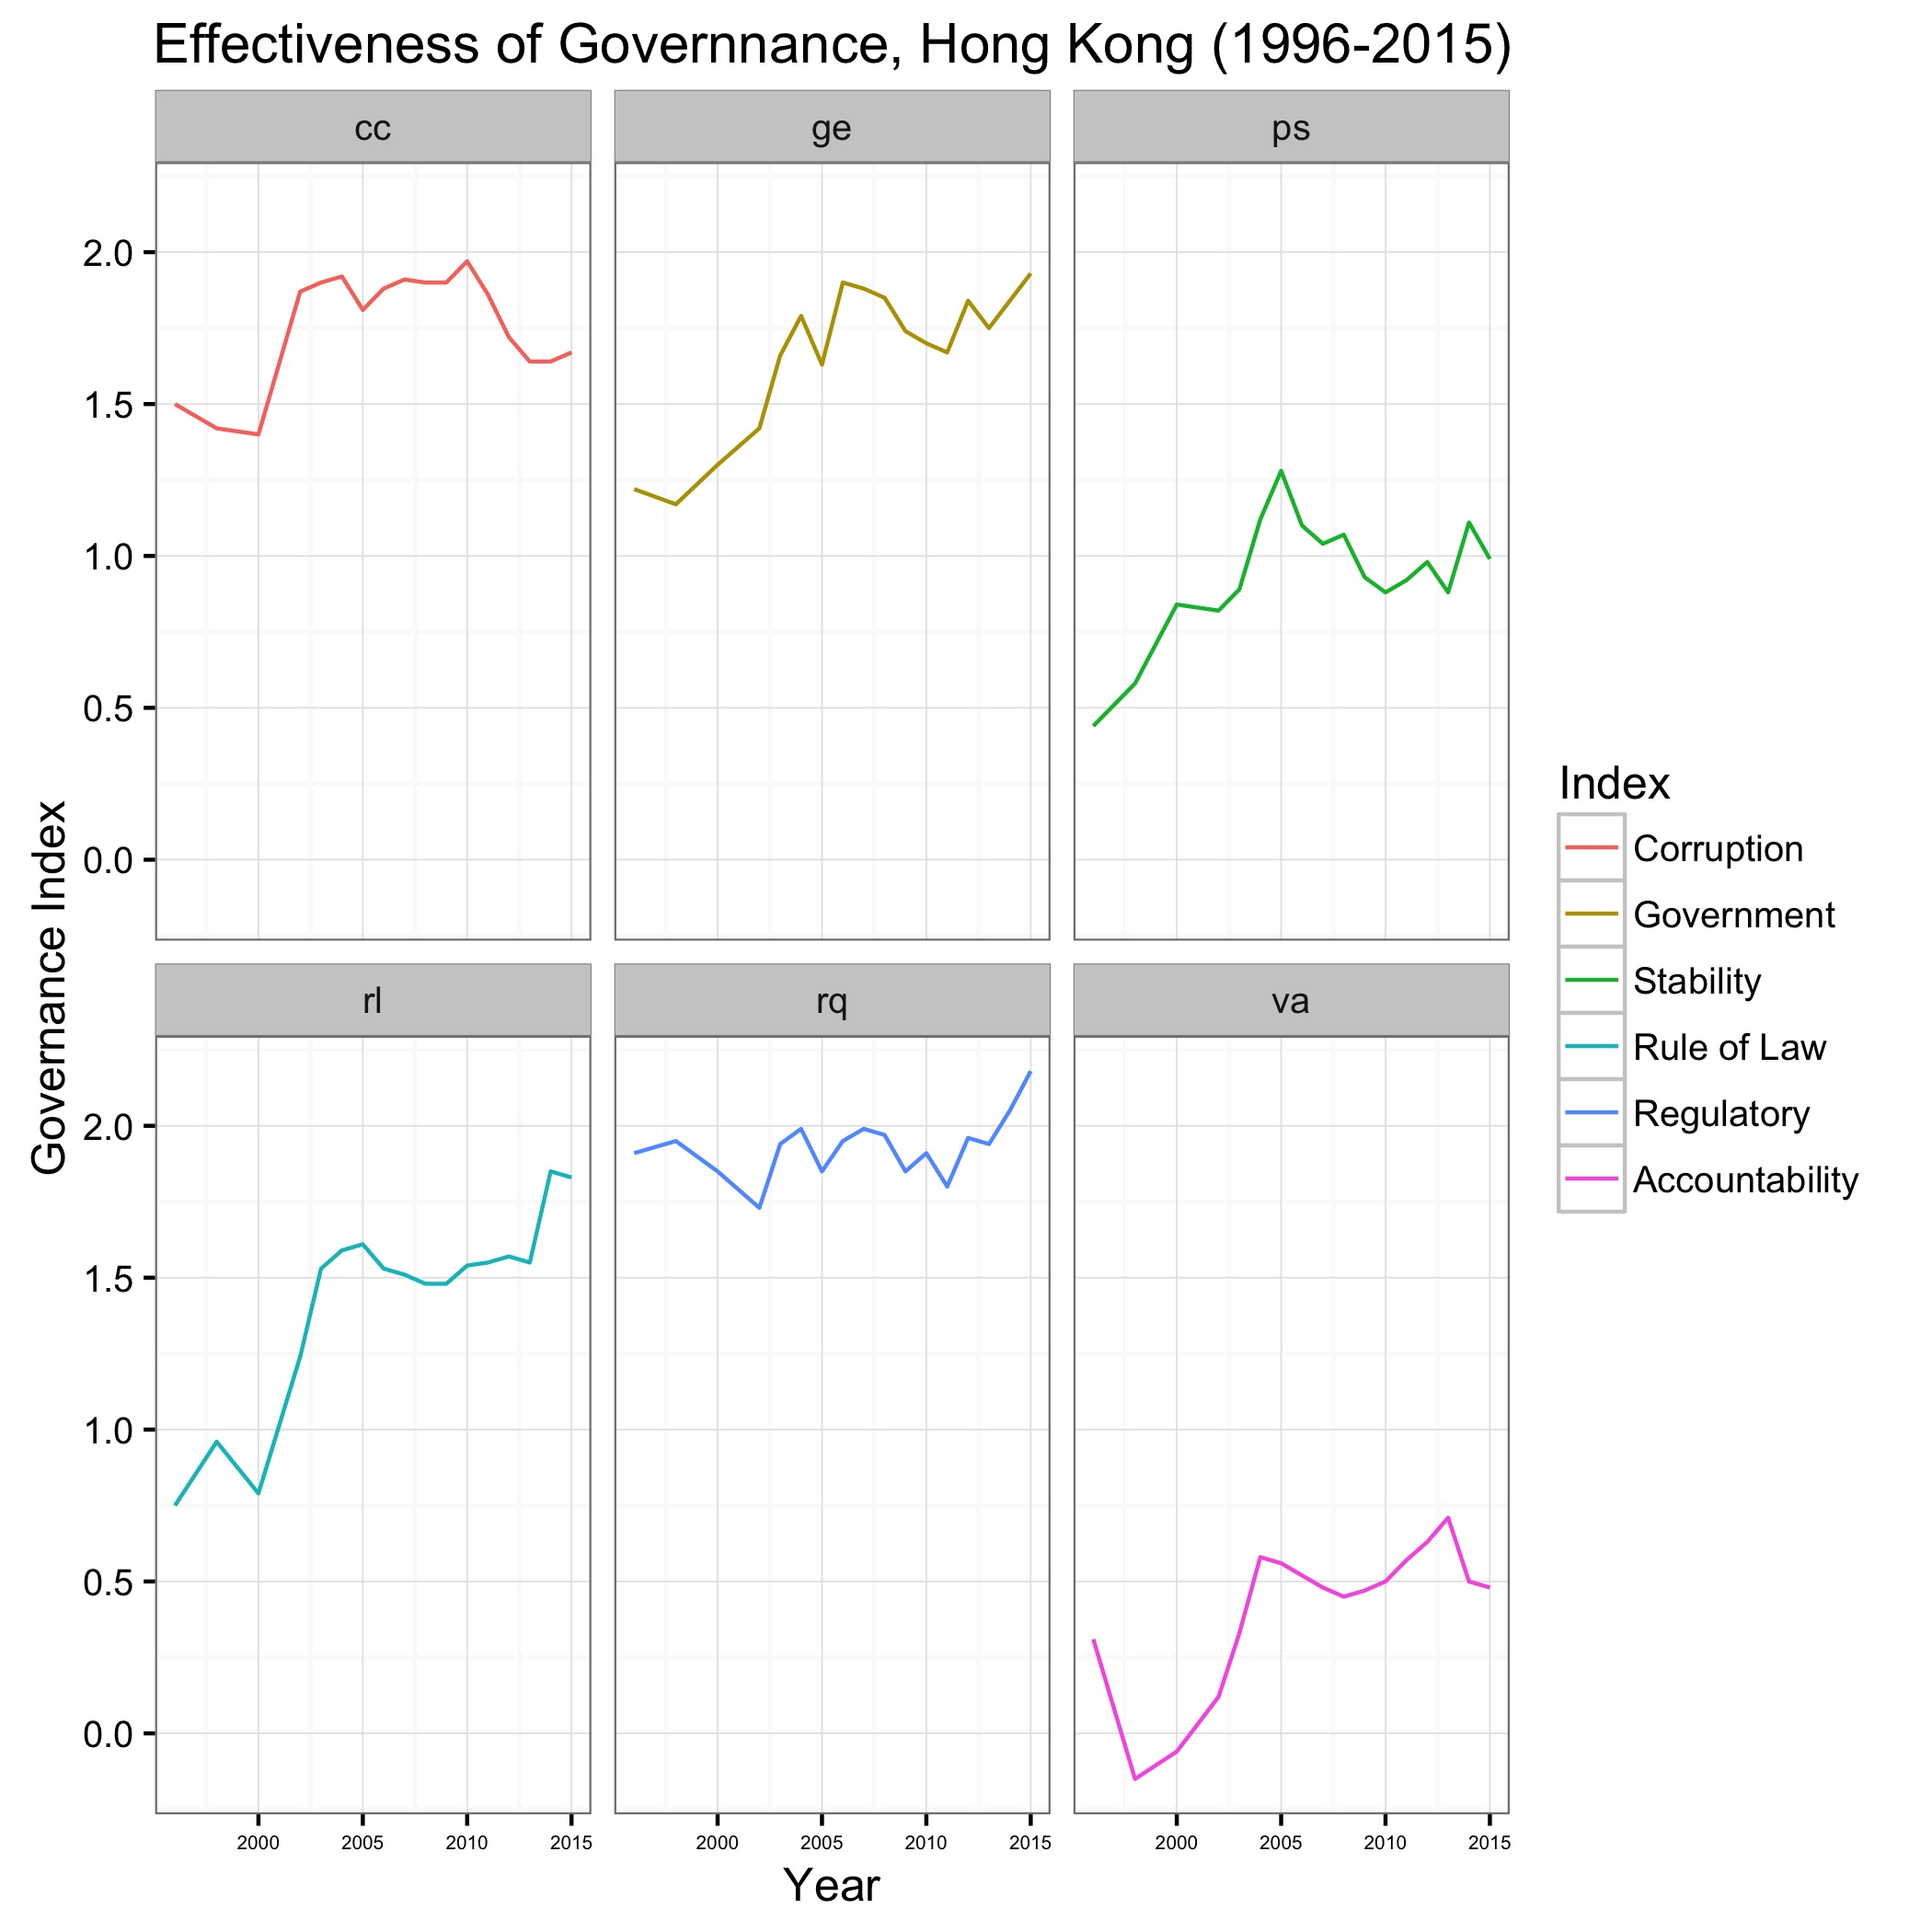
\includegraphics[scale=0.2]{../Plots_Figs/hk_plot.jpeg} 
\caption{Effectiveness of Governance}
\end{figure}
%%%%%%%%%%%%%%%
\begin{figure}
	\centering
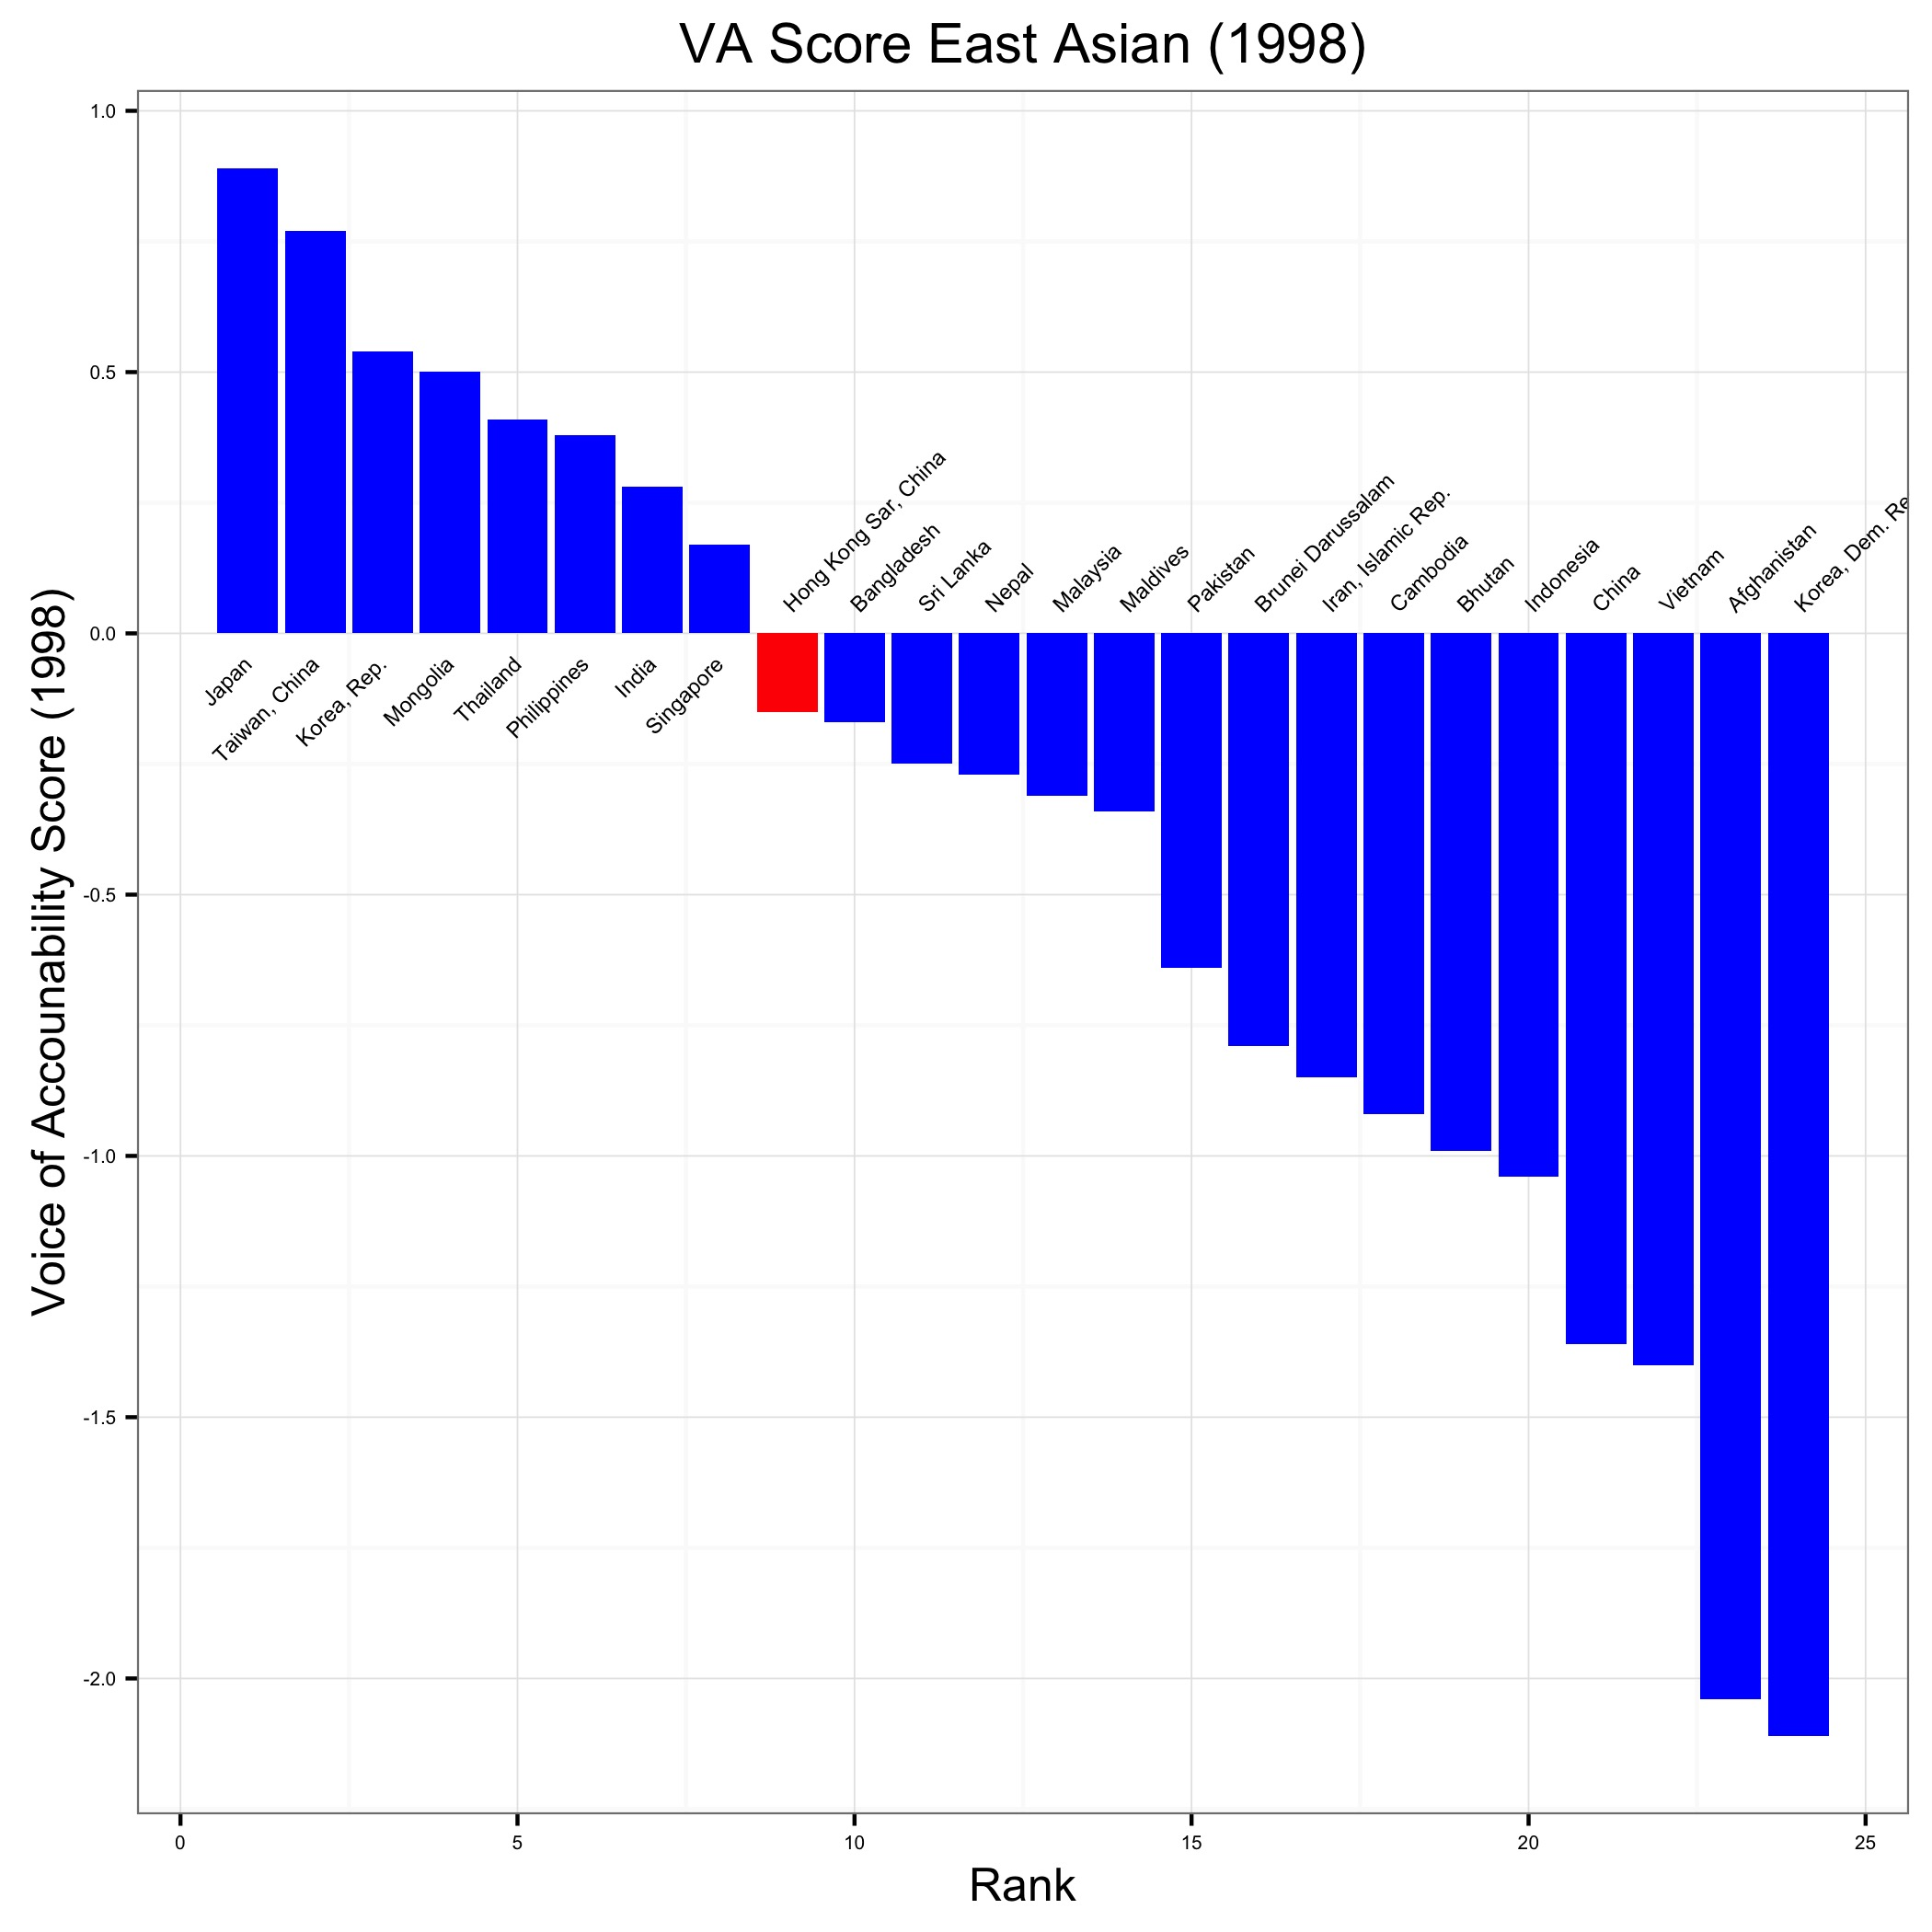
\includegraphics[scale=0.2]{../Plots_Figs/ea_va_98.jpeg} 
\caption{Accountability Score, 1998}
\end{figure}
%%%%%%%%%%%%%%%
\begin{figure}
	\centering
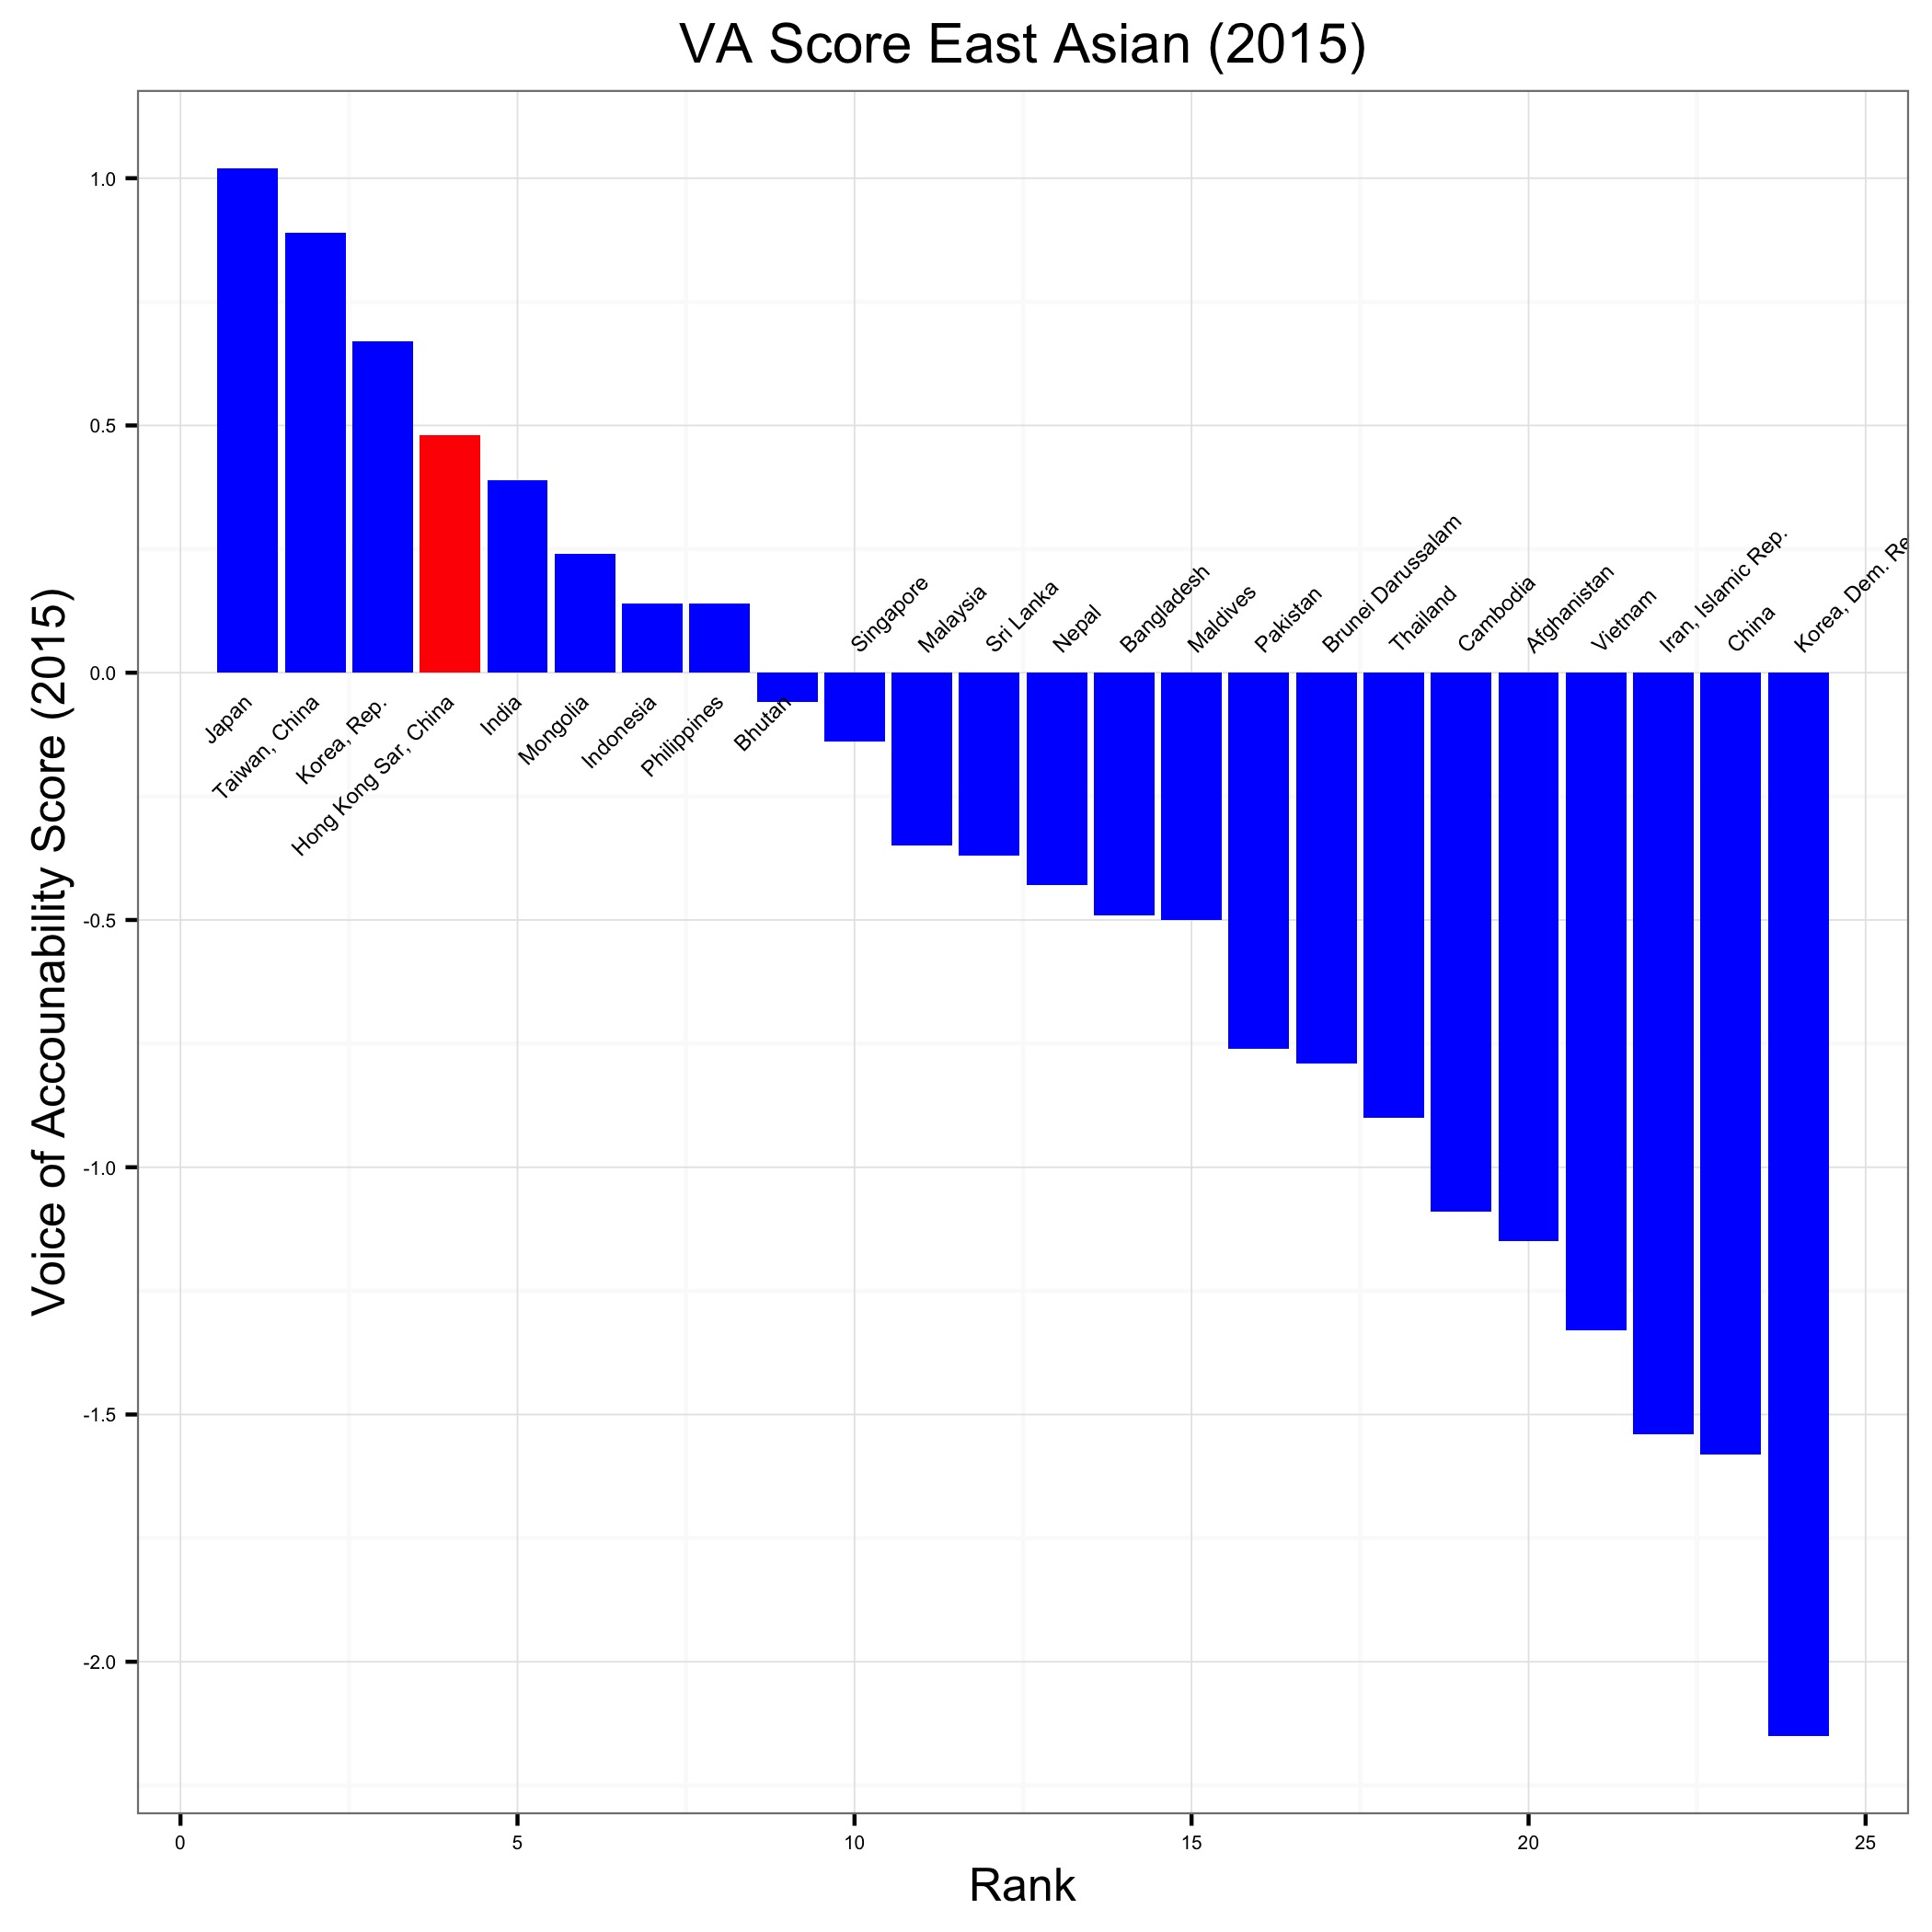
\includegraphics[scale=0.2]{../Plots_Figs/ea_va_15.jpeg} 
\caption{Accoutability Score, 2015}
\end{figure}

\begin{figure}
	\centering
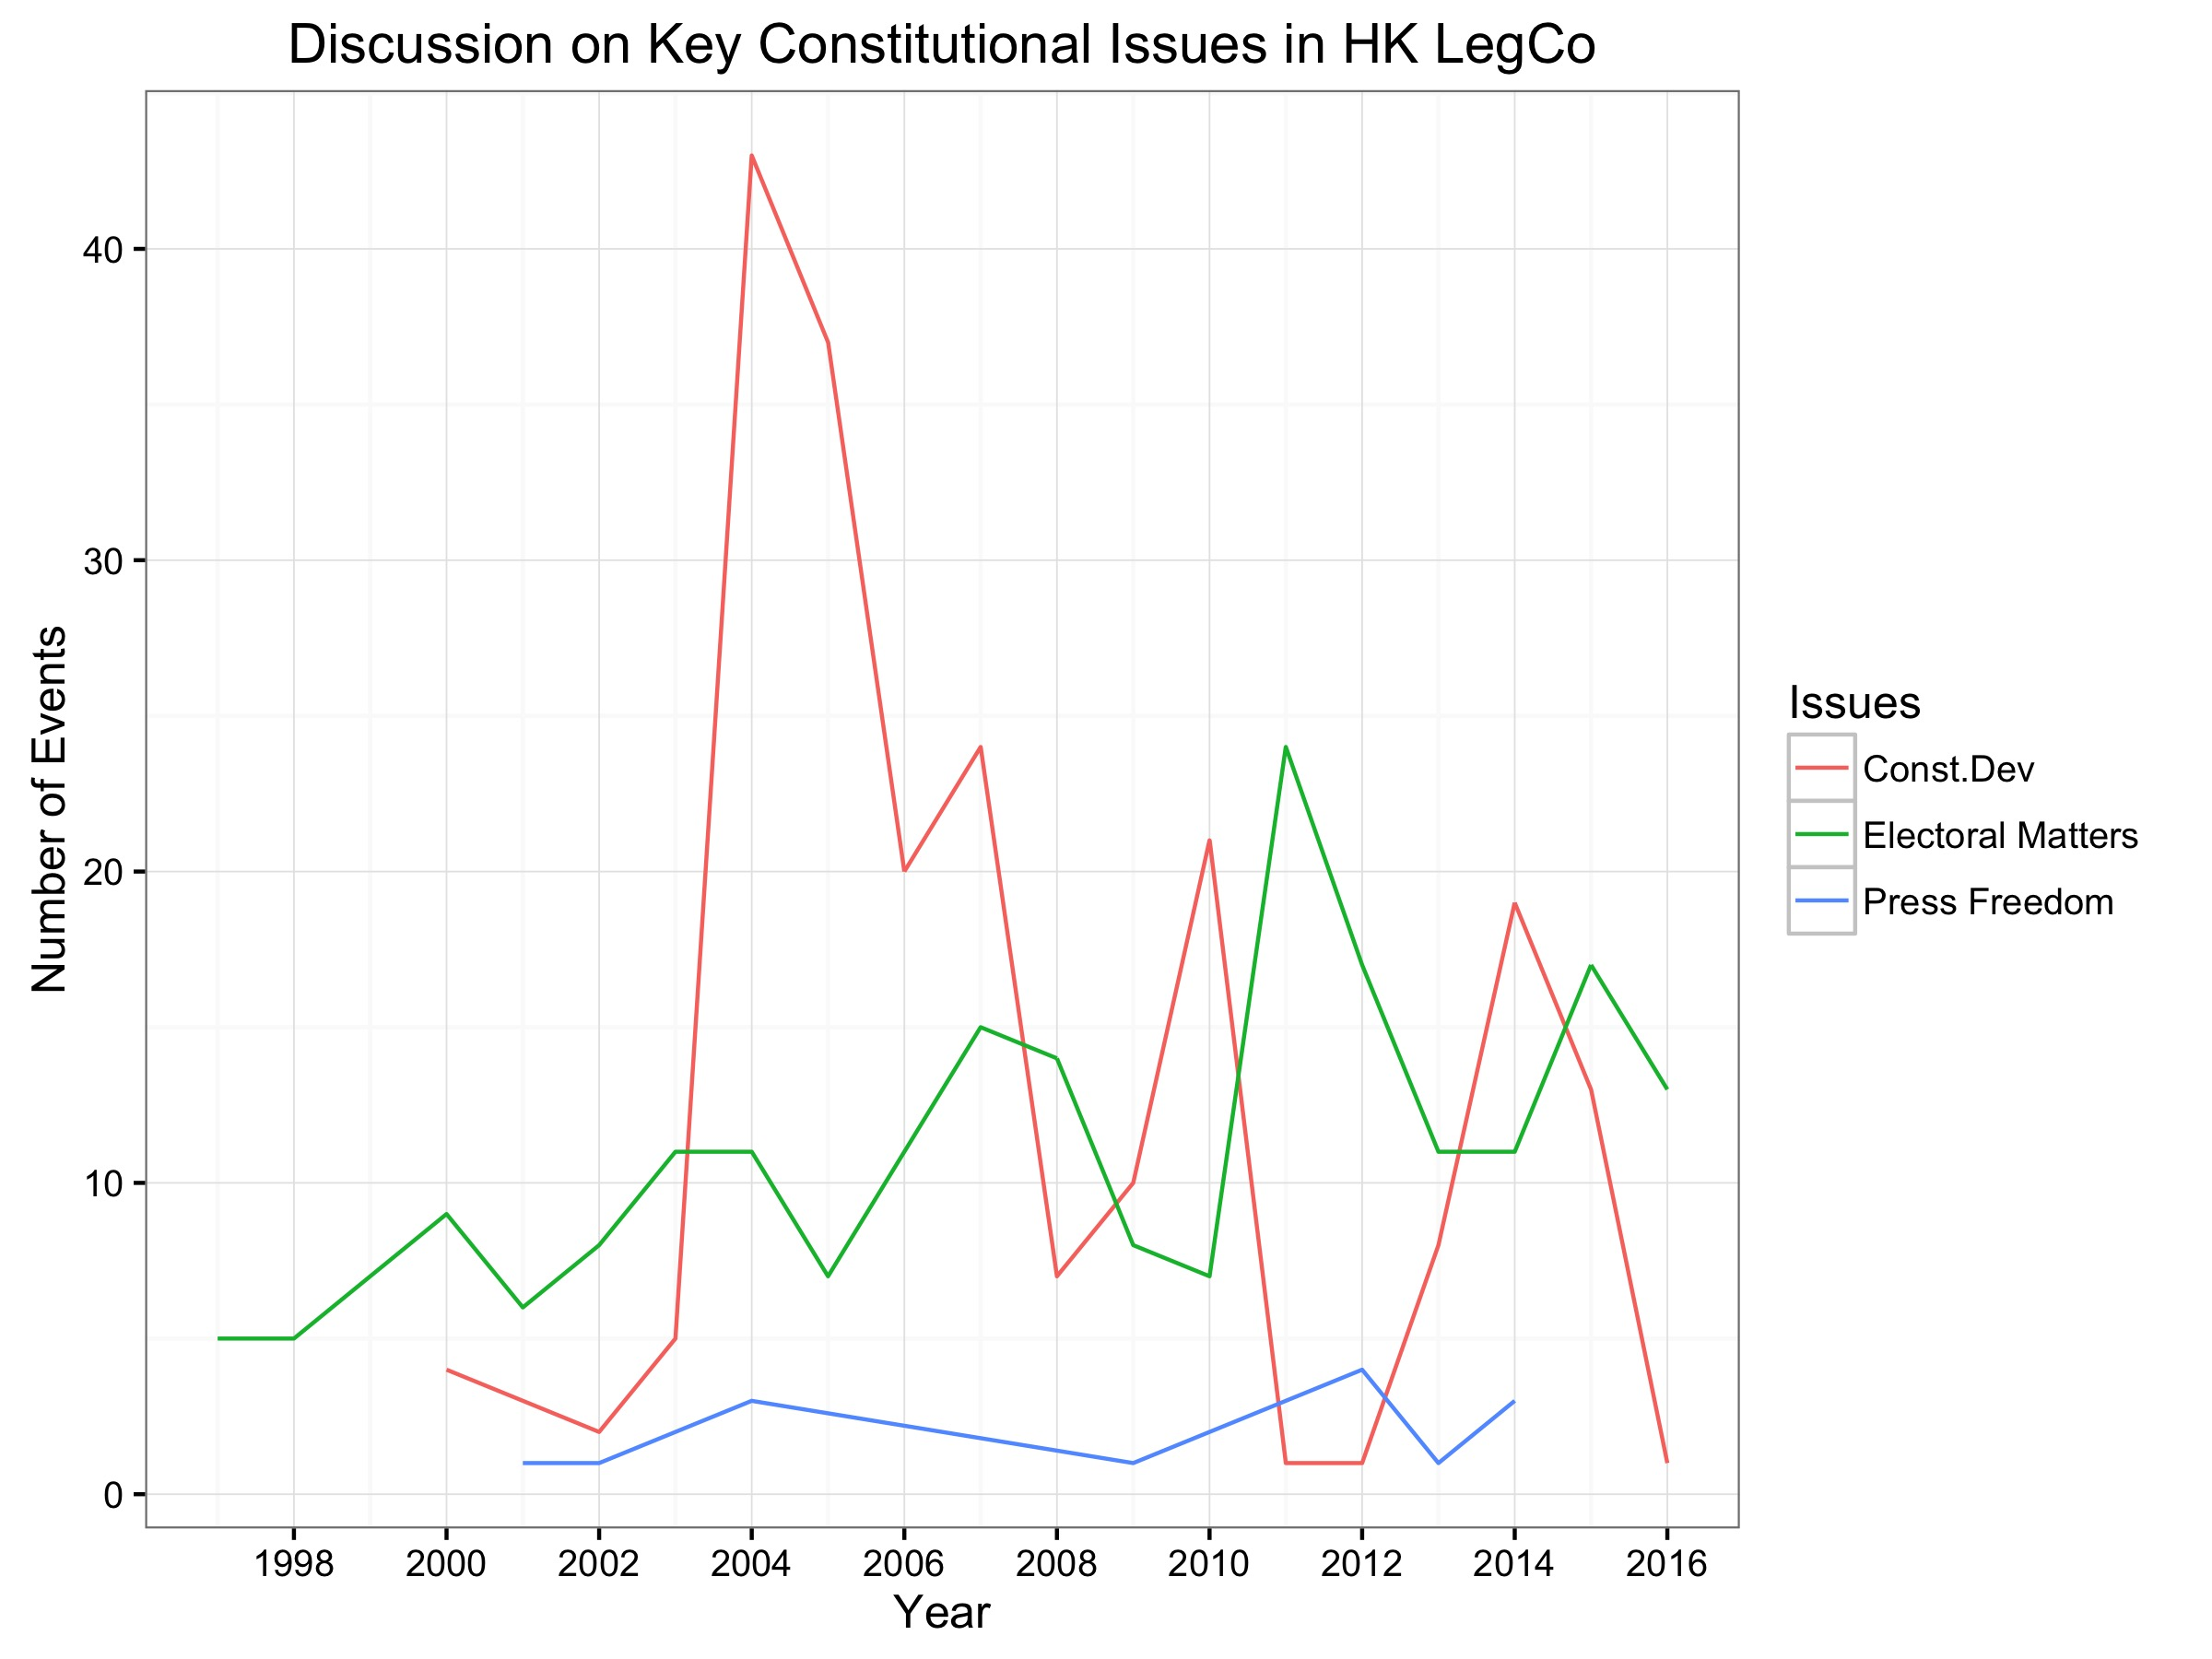
\includegraphics[scale=0.2]{../Plots_Figs/keyissu.jpeg} 
\caption{Numer of Discussions on Key Constitutional Issues}
\end{figure}

\begin{figure}
	\centering
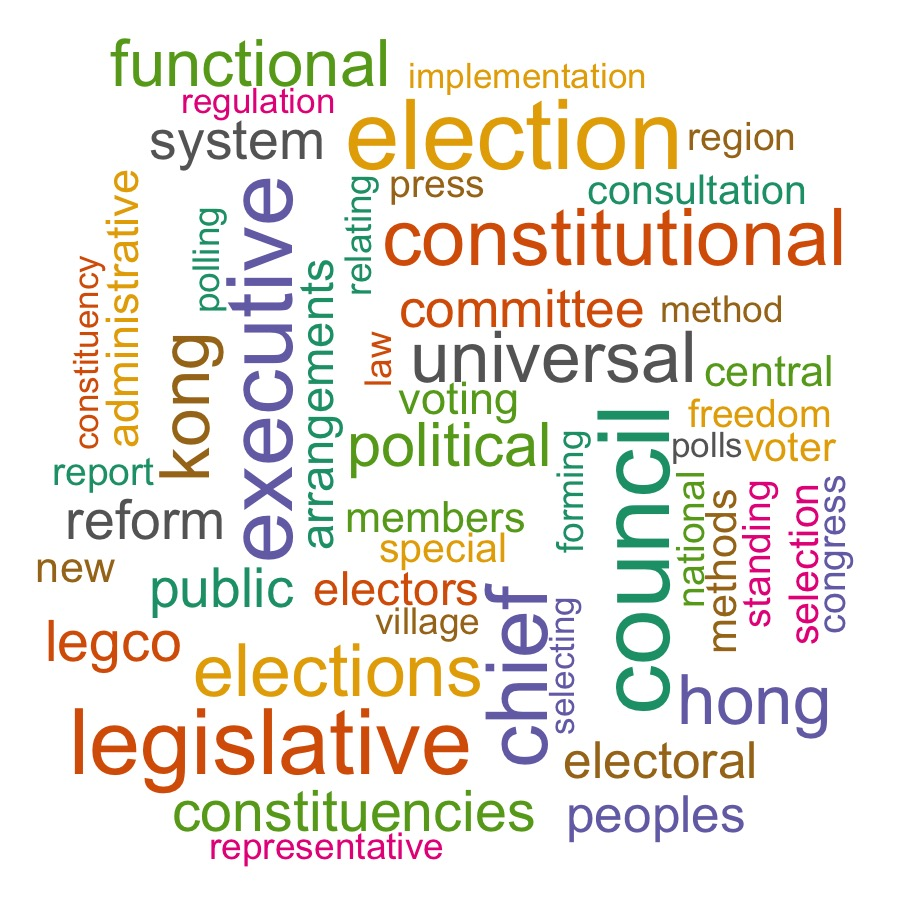
\includegraphics[scale=0.35]{../Plots_Figs/wc-motion.jpeg} 
\caption{Word Cloud of Motion Topics}
\end{figure}



\end{document}